\begin{center}
	\Large
	Uden hjælpemidler	
\end{center}
%
%
%
%
%
\begin{opgavetekst}{Opgave 1}
	En linje $l$ er givet ved
	\begin{align*}
		l: \ 5(x - 2) - 8(y+1) = 0.
	\end{align*}
\end{opgavetekst}
%
%
\begin{delopgave}{1}
	Bestem en normalvektor til $l$ samt et punkt, der ligger på linjen.
\end{delopgave}
\begin{meretekst}
	En anden linje $m$ har vektoren $\vv{r}$ givet ved
	\begin{align*}
		\vv{r} = 
		\begin{pmatrix}
			4 \\ -3		
		\end{pmatrix}
	\end{align*}
	som retningsvektor og går gennem punktet $(6,7)$.
\end{meretekst}
\begin{delopgave}{2}
	Opskriv linjens ligning for $m$.
\end{delopgave}
\begin{delopgave}{3}
	Bestem skæringspunktet mellem $l$ og $m$.
\end{delopgave}
%
%
%
%
%
\begin{opgavetekst}{Opgave 2}
	En cirkel er givet ved ligningen
	\begin{align*}
		x^2 - 4x + y^2 + 10y = 71.
	\end{align*}
\end{opgavetekst}
%
%
\begin{delopgave}{1}
Bestem centrum og radius for cirklen. 
\end{delopgave}
%
%
%
%
%
\begin{opgavetekst}{Opgave 3}
	På Figur \ref{fig:vektorer} kan vi se to vektorer $\vv{a}$ og $\vv{b}$ samt et skraveret område $M$.
	\begin{figure}[H]
		\centering
		\begin{tikzpicture}
			\begin{axis}[
				axis lines = center, 
				xmin = -1.5, xmax = 7.5, 
				ymin = -1.5, ymax = 7.5, 
				x = 1.0cm, y = 1.0cm,
				grid,
				xlabel = $x$, ylabel = $y$
			]
				\draw[-{Stealth[scale=1.5]}, thick, color = teal] (axis cs: 1,5) -- (axis cs: 5,7) node[midway, xshift = -7pt, yshift = 7pt] {$\vv{a}$};
				\draw[-{Stealth[scale=1.5]}, thick, color = teal] (axis cs: 1,5) -- (axis cs: 3,2) node[midway, xshift = 7pt, yshift = 7pt] {$\vv{b}$};
				\fill[olive,nearly transparent] (axis cs: 1,5) -- (axis cs: 5,7) -- (axis cs:7,4) -- (axis cs: 3,2) -- cycle;
				\node[color = teal] at (axis cs: 4,4.5) {$M$};
			\end{axis}
		\end{tikzpicture}
		\caption{To vektorer.}
		\label{fig:vektorer}
	\end{figure}
	\phantom{h}
\end{opgavetekst}
\begin{delopgave}{1}
	Afgør, om vektorerne $\vv{a}$ og $\vv{b}$ er orthogonale.
\end{delopgave}
\begin{delopgave}{2}
	Bestem arealet af det skraverede område $M$. 
\end{delopgave}
%
%
%
%
%
\begin{opgavetekst}{Opgave 4}
\end{opgavetekst}
\begin{delopgave}{1}
	Isolér L i udtrykket
	\begin{align*}
		V = 2\cdot 5^{L-7}.
	\end{align*}
\end{delopgave}
\begin{delopgave}{2}
	Reducér følgende udtryk
	\begin{align*}
		\frac{4a(a-b)^2 - 4a^3 - 4ab^2}{2ab^2}.
	\end{align*}
\end{delopgave}
%
%
%
%
%
\begin{opgavetekst}{Opgave 5}
	Grafen for funktionen $f$ kan ses på Figur \ref{fig:areal}
	\begin{figure}[H]
		\centering
		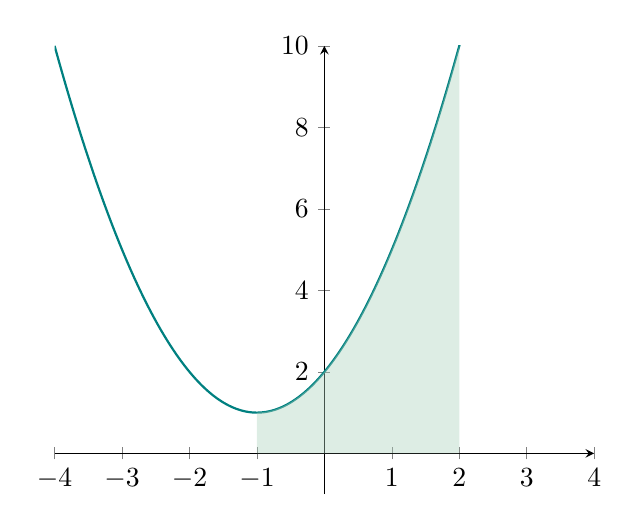
\begin{tikzpicture}
		\begin{axis}
			[
			axis lines = center, 
			xmin = -4, xmax = 4, 
			ymin = -1, ymax = 10,
			xtick = {-5,-4,...,4,5}, ytick = {-12,-10,...,10,12},
			]
				\addplot[color = teal, thick, domain = -4:4, samples = 400] {x^2 + 2*x + 2};
				\fill
				[
				color = SeaGreen!40,
				opacity = 0.4,
				variable = \x, 
				domain = -1:2,
				]	
				(axis cs: 2,0) -- (axis cs: -1,0) --
				plot(axis cs: \x, {(\x)^2 + 2*\x + 2}) --  cycle;
		\end{axis}
		\end{tikzpicture}
		\caption{Graf for $f$ samt markeret område under grafen for $f$.}
		\label{fig:areal}
	\end{figure}
	\phantom{h}
\end{opgavetekst}
\begin{delopgave}{1}
	Bestem arealet under grafen for $f$ markeret på Figur \ref{fig:areal}.
\end{delopgave}
%
%
%
%
%
\begin{opgavetekst}{Opgave 6}
	Funktionen $g$ er givet ved
	\begin{align*}
		g(x) = \frac{7}{x} + 5x
	\end{align*}
	for $x > 0$. 
\end{opgavetekst}
%
%
\begin{delopgave}{1}
	Bestem en stamfunktion til $g$, der går gennem punktet $(1,2)$. 
\end{delopgave}
%
%
%
%
%
\begin{opgavetekst}{Opgave 7}
	En funktion $h$ er givet ved
	\begin{align*}
		h(x) = \sqrt{x^2 - 2x + 12}
	\end{align*}
\end{opgavetekst}
%
%
\begin{delopgave}{1}
	Bestem tangenthældningen for $h$ i punktet $(4,h(4))$. 
\end{delopgave}
%
%
%
%
%
\newpage
\begin{center}
	\Large
	Med hjælpemidler
\end{center}
%
%
\begin{opgavetekst}{Opgave 8}
	To linjer $l$ og $m$ er givet ved henholdsvis
	\begin{align*}
		&l: \ -9(x - 15) -7(y - 4) = 0, \\
		&m: \ 
		\begin{pmatrix}
			x \\ y	
		\end{pmatrix}
		=
		\begin{pmatrix}
			13 \\ k
		\end{pmatrix}
		+ t
		\begin{pmatrix}
			-5 \\ 19
		\end{pmatrix}.
	\end{align*}
\end{opgavetekst}
\begin{delopgave}{1}
	Bestem tallet $k$, så $l$ og $m$ skærer hinanden i punktet $(29,-14)$.
\end{delopgave}
%
%
%
%
%
\begin{opgavetekst}{Opgave 9}
	To vektorer $\vv{a}$ og $\vv{b}$ kan ses på Figur \ref{fig:proj}.
	\begin{figure}[H]
		\centering
		\begin{tikzpicture}
		\begin{axis}
			[
			axis lines = center,
			xmin = -5, xmax = 7,
			ymin = -5, ymax = 7,
			y = 1cm, x = 1cm,
			grid = both, 
			]
				\draw[-{Stealth[scale=1.5]}, color = teal, thick] (axis cs: -4,-3) -- (axis cs: 6,3)
				node[midway, anchor = south east] {$\vv{b}$};				
				\draw[-{Stealth[scale=1.5]}, color = olive, thick] (axis cs: -4,-3) -- (axis cs: -1,5) 
				node[midway, anchor = south east] {$\vv{a}$};
		\end{axis}	
		\end{tikzpicture}
		\caption{To vektorer}
		\label{fig:proj}
	\end{figure}
	\phantom{h}
\end{opgavetekst}
\begin{delopgave}{1}
	Bestem koordinatsættet til projektionsvektoren $\vv{b_{\vv{a}}}$.
\end{delopgave}
\begin{meretekst}
	En linje $l$ har $\vv{a}$ som normalvektor og går gennem punktet $(-3,-4)$.
\end{meretekst}
\begin{delopgave}{2}
	Bestem afstanden mellem $l$ og punktet $(2,2)$. 
\end{delopgave}
%
%
%
%
%
\begin{opgavetekst}{Opgave 10}
	\begin{center}
		
\includegraphics[width=0.6\textwidth]{Billeder/beer}
	\end{center}
	Henover en sommersæson finder en bar-ejer ud af, at salget af øl i baren kan beskrives ved funktionen 
	\begin{align*}
		f(x) = -0.02705x^2 +5.5150x + 230, \ 0 \leq x \leq 200
	\end{align*}
	hvor $x$ er antallet af dage siden sommersæsonens begyndelse og $f$ er antallet af solgte øl på dagen.
\end{opgavetekst}
\begin{delopgave}{1}
	Bestem $f'(20)$ og giv en fortolkning af dette tal. 
\end{delopgave}
\begin{delopgave}{2}
	Bestem det gennemsnitlige antal øl, barejeren i følge modellen sælger om dagen henover sæsonens 200 dage.
\end{delopgave}
\begin{delopgave}{3}
	Hvor mange øl sælger ejeren i følge modellen henover sæsonens 200 dage?
\end{delopgave}
%
%
%
%
%
\begin{opgavetekst}{Opgave 11}
	\begin{center}
		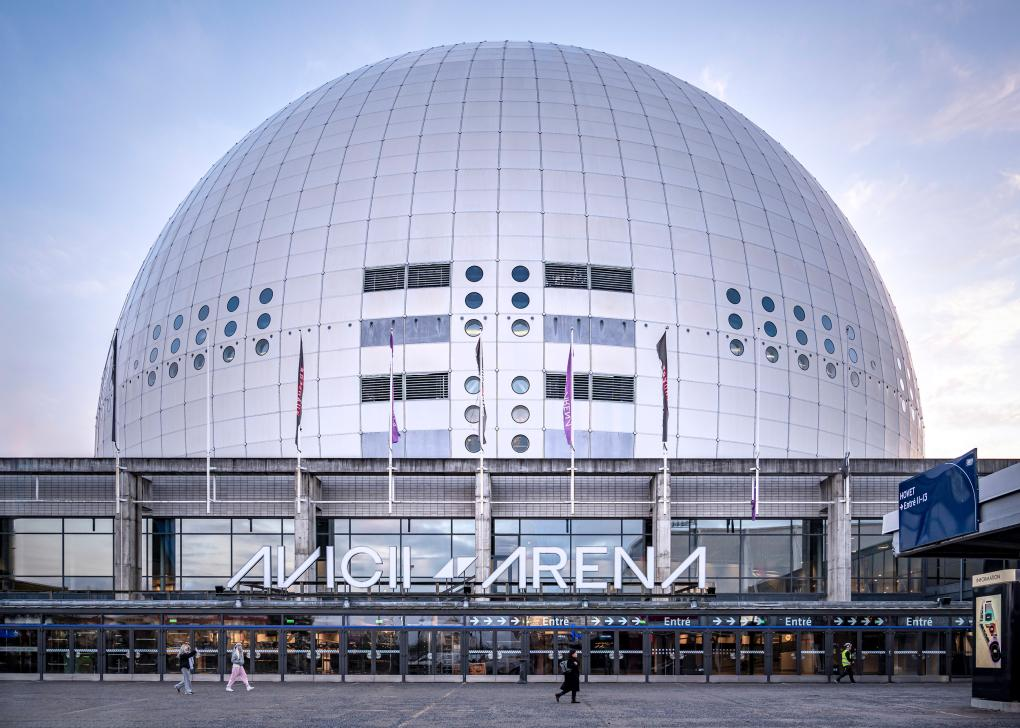
\includegraphics[width=0.6\textwidth]{Billeder/globen}
	\end{center}	
	Den største sfæriske bygning i verden var indtil 2023 Avicii Arena i Stockholm, der typisk blot kaldes globen.
	Tværsnittet af bygningen kan tilnærmelsesvist beskrives af funktionen $h$ givet ved
	\begin{align*}
		h(x) = \sqrt{3025 - x^2},
	\end{align*}
	hvor $x$ er afstanden fra bygningens centrum og $h$ er højden på stedet. Alle længder er i meter. 
\end{opgavetekst}
%
%
\begin{delopgave}{1}
	Tegn grafen for $h$ på intervallet $[-55,55]$. 	
\end{delopgave}
\begin{delopgave}{2}
	Bestem rumfanget af Avicii Arena.
\end{delopgave}
